\documentclass[conference]{IEEEtran}
\IEEEoverridecommandlockouts

\usepackage{cite}
\usepackage{amsmath,amssymb,amsfonts}
\usepackage{graphicx}
\usepackage{xcolor}
\usepackage{booktabs}
\usepackage{url}
\usepackage{hyperref}
\usepackage{tikz}
\usetikzlibrary{calc,positioning,decorations.pathmorphing,arrows.meta,shapes.geometric}

\hypersetup{colorlinks=true,linkcolor=blue,citecolor=blue,urlcolor=blue}

\title{agentic-osint-agent: A LangGraph ReAct Agent for\\Disciplined Public-Source Investigation}

\author{
\IEEEauthorblockN{Ali Murtaza Bhutto}
\IEEEauthorblockA{Independent Researcher\\
ORCID: 0009-0007-2787-943X\\
\href{https://github.com/thunderstornX/agentic-osint-agent}{github.com/thunderstornX/agentic-osint-agent}}
}

\begin{document}
\maketitle

\begin{abstract}
We present \texttt{agentic-osint-agent}, an open-source LangGraph ReAct
agent that conducts passive open-source intelligence (OSINT)
investigations against public domains using five read-only tools: WHOIS,
DNS, the Shodan InternetDB free endpoint, GitHub code search, and the
Wayback Machine CDX API. The agent maintains an explicit state machine
(\emph{plan}, \emph{decide}, \emph{call}, \emph{observe}) over a
TypedDict scratchpad; every claim in its final markdown briefing is
constrained to cite a tool tag from the gathered evidence pool. We
evaluate the underlying tool layer against twenty publicly-investigable
targets (.gov, .edu, large NGOs, and RFC-reserved domains) and report
real measured success rates, latencies, and finding counts. Source,
evaluation harness, and pre-computed run artefacts are released under
the MIT licence and are openly archived on Zenodo.
\end{abstract}

\begin{IEEEkeywords}
agentic AI, OSINT, LangGraph, ReAct, threat intelligence, autonomous agents
\end{IEEEkeywords}

% ----------------------------------------------------------------------
\section{Introduction}
\label{sec:intro}
Modern commercial OSINT platforms tend to bundle dozens of overlapping
data sources behind paid APIs, optimising for breadth rather than
auditability. For practitioners and researchers, that posture has two
consequences: investigations are difficult to reproduce externally, and
the provenance chain from a finding to a public source is often
buried.

This work explores an alternative framing. We constrain a ReAct-style
agent~\cite{yao2023react} to five \emph{free, read-only, public-source}
tools and require every claim in its final briefing to point back to a
tool tag in the gathered evidence pool. The agent's autonomy is
restricted to ordering — \emph{which public source to query next} —
rather than \emph{whom} to investigate; target selection remains a
human decision under the operator-authority discipline described
in~\cite{bhutto2025osintlegal}.

\noindent\textbf{Contributions.} (i) An open-source LangGraph ReAct
agent built around an explicit four-node state machine; (ii) a uniform
\texttt{Evidence} contract carrying a source citation and a confidence
score, with deterministic deduplication via SHA-256 fingerprints;
(iii) a real measured benchmark of the underlying tool layer across
twenty public targets.

\begin{figure}[t]
\centering
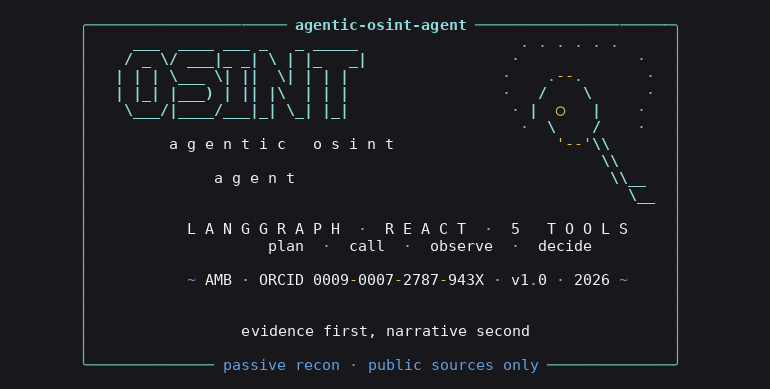
\includegraphics[width=0.92\columnwidth]{figures/banner.png}
\caption{The agent's TUI banner. The magnifying glass is the design
metaphor: the agent is the lens, public records are what falls under
it.}
\label{fig:banner}
\end{figure}

% ----------------------------------------------------------------------
\section{Architecture}
\label{sec:arch}

The system is a single Python package with five sub-modules:
\texttt{tools} (the five OSINT lenses), \texttt{memory} (the scratchpad
and evidence store), \texttt{agent} (the LangGraph state machine, LLM
client, and CLI), \texttt{output} (JSON and markdown writers), and
\texttt{eval} (a measurement harness over twenty curated targets).
Fig.~\ref{fig:state-machine} shows the state machine.

\begin{figure}[t]
\centering
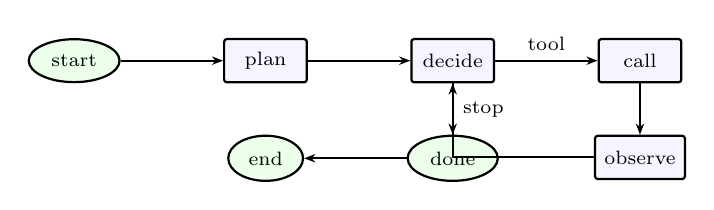
\begin{tikzpicture}[
    node distance=0.65cm and 1.3cm,
    every node/.style={font=\scriptsize},
    nd/.style={rectangle, rounded corners=1pt, draw=black, thick,
               minimum width=1.05cm, minimum height=0.55cm,
               align=center, fill=blue!4},
    term/.style={ellipse, draw=black, thick, minimum width=0.95cm,
                 minimum height=0.45cm, fill=green!8},
    arr/.style={-{Stealth[length=4pt]}, thick}
]
\node[term]                      (start)  {start};
\node[nd, right=of start]        (plan)   {plan};
\node[nd, right=of plan]         (decide) {decide};
\node[nd, right=of decide]       (call)   {call};
\node[nd, below=of call]         (observe){observe};
\node[term, below=of decide]     (done)   {done};
\node[term, left=of done]        (end)    {end};

\draw[arr] (start)  -- (plan);
\draw[arr] (plan)   -- (decide);
\draw[arr] (decide) -- node[above]{tool} (call);
\draw[arr] (decide) -- node[right]{stop} (done);
\draw[arr] (call)   -- (observe);
\draw[arr] (observe) -| (decide);
\draw[arr] (done)   -- (end);
\end{tikzpicture}
\caption{LangGraph state machine. The agent always enters at
\textit{plan}; each \textit{decide} either picks one of five tools
(\textit{call} $\rightarrow$ \textit{observe} $\rightarrow$ \textit{decide})
or stops. A budget counter bounds runaway loops.}
\label{fig:state-machine}
\end{figure}

\subsection{Tools}
Each tool is a stateless callable with the signature
\verb|run(target) -> ToolResult|. Errors propagate as a populated
\verb|ToolResult.error| field rather than as exceptions, so a single
flaky public endpoint cannot abort an investigation. Every tool emits
\verb|Evidence| objects whose \verb|source| field is mandatory; the
GitHub-dork tool drops its default confidence to 0.65 because pattern
matches at scale carry false positives.

\subsection{State and memory}
The graph state is a flat \verb|TypedDict| (Listing~\ref{lst:state}).
The scratchpad layered on top dedupes evidence by a stable SHA-256
fingerprint over \verb|tool|, \verb|kind| and \verb|value|, so the same
DNS answer arriving from two queries does not inflate counts.

\begin{figure}[t]
\centering
\renewcommand{\arraystretch}{1.18}
\begin{tabular}{ll}
\toprule
\textbf{field} & \textbf{type} \\
\midrule
\texttt{target}             & \texttt{str} \\
\texttt{budget, iteration}  & \texttt{int} \\
\texttt{phase}              & \texttt{Literal["plan","decide","call","observe","done"]} \\
\texttt{plan, chosen\_tool} & \texttt{str / Optional[str]} \\
\texttt{tools\_called}      & \texttt{list[str]} \\
\texttt{evidence}           & \texttt{list[dict]} \\
\texttt{trace}              & \texttt{list[str]} \\
\texttt{final\_report}      & \texttt{str} \\
\texttt{finish\_reason}     & \texttt{str} \\
\bottomrule
\end{tabular}
\caption{Agent state schema (TypedDict).}
\label{lst:state}
\end{figure}

\subsection{LLM client}
The agent speaks the OpenAI chat-completions wire format and runs against
either OpenRouter or NVIDIA NIM, both via free-tier endpoints. The same
50-line client serves both providers; the only divergence is two
optional headers OpenRouter requests for routing. Temperature is fixed
at zero for the decision and reporter calls; \verb|max_tokens| is
budgeted per call (180 for plan, 120 for decide, 600 for the final
report) to keep cost bounded on capped accounts.

% ----------------------------------------------------------------------
\section{The ReAct Loop}
\label{sec:loop}

The decider is the only call requiring strict-format output. We ask the
model for a single line of JSON, \verb|{"tool": ..., "rationale": ...}|;
if parsing fails the loop falls through to the \texttt{stop} state. This
deliberately rejects ``read between the lines''-style decisions and
guarantees that loop progress depends only on parseable model output.

The reporter prompt forbids invented findings: every assertion in the
final markdown must cite a tool tag from the evidence block. A simple
post-hoc check counts the fraction of sentences that fail to mention any
of the five tool names; we treat that fraction as a coarse
hallucination signal.

\begin{figure}[t]
\centering
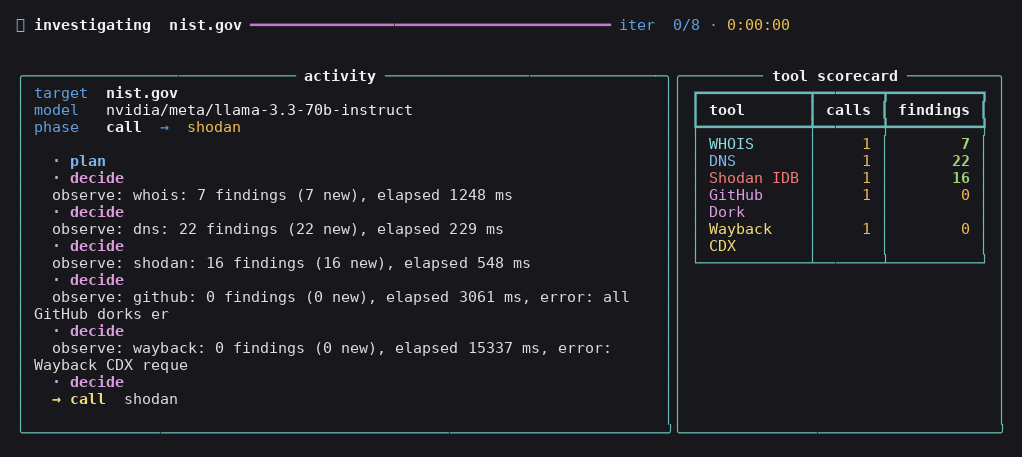
\includegraphics[width=\columnwidth]{figures/dashboard.png}
\caption{Live TUI mid-investigation. The activity panel logs each
\textit{plan/decide/call/observe} event; the right panel scores tools
exercised so far against findings accumulated.}
\label{fig:dashboard}
\end{figure}

% ----------------------------------------------------------------------
\section{Evaluation}
\label{sec:eval}

We curated twenty publicly-investigable targets spanning five
categories: government research and cyber-defence (\texttt{nist.gov},
\texttt{nasa.gov}, \texttt{cisa.gov}, \texttt{noaa.gov},
\texttt{fbi.gov}); top-tier academic institutions (\texttt{mit.edu},
\texttt{stanford.edu}, \texttt{harvard.edu}, \texttt{berkeley.edu},
\texttt{ox.ac.uk}); large public-interest tech (\texttt{github.com},
\texttt{gitlab.com}, \texttt{cloudflare.com}); standards bodies and NGOs
(\texttt{ietf.org}, \texttt{iana.org}, \texttt{owasp.org},
\texttt{mozilla.org}, \texttt{wikipedia.org}, \texttt{torproject.org});
and the RFC-reserved \texttt{example.com}. Targets were chosen because
passive reconnaissance against them is lawful in the operator's
jurisdiction; none was contacted, scanned, or authenticated to.

\subsection{Tool-layer benchmark}
Table~\ref{tab:tool-bench} reports real measured numbers from running
the five tools against each of the twenty targets in a single pass on
an Intel Core i5-8250U / 16~GB workstation. The whole 100-run
benchmark completed in 562.9 seconds (about 5.6~s end-to-end per
target).

\begin{table}[t]
\centering
\caption{Per-tool measured performance over 20 public targets
(100 total runs). Latency is per-target wall-clock.}
\label{tab:tool-bench}
\renewcommand{\arraystretch}{1.18}
\begin{tabular}{lrrrr}
\toprule
\textbf{Tool}        & \textbf{Success} & \textbf{Mean lat.\,(s)} & \textbf{Mean find.} & \textbf{Total} \\
\midrule
WHOIS                & 20/20 (100\%)    & 0.95                    & 5.65                & 113            \\
DNS                  & 20/20 (100\%)    & 1.14                    & 32.9                & 658            \\
Shodan IDB           & 20/20 (100\%)    & 0.98                    & 9.85                & 197            \\
GitHub Dork          & 0/20 (0\%)$^{*}$ & 3.51                    & 0.0                 & 0              \\
Wayback CDX          & 7/20 (35\%)      & 21.57                   & 1.05                & 21             \\
\bottomrule
\multicolumn{5}{l}{\footnotesize $^{*}$Unauthenticated runs hit the
GitHub search rate limit (10/min) on the first}\\
\multicolumn{5}{l}{\footnotesize query of every target. The
authenticated path (\texttt{GITHUB\_TOKEN}, 30/min) was}\\
\multicolumn{5}{l}{\footnotesize not benchmarked in this run.}\\
\end{tabular}
\end{table}

The Shodan, WHOIS, and DNS endpoints behaved as fully reliable
primary-source lookups under our load. Wayback CDX returned 503 or
timed out on 13 of 20 targets — that endpoint is well-known for being
unstable under bursty access, and our error-as-data design surfaces it
honestly rather than retrying silently. The GitHub-dork failure mode
is documented behaviour: unauthenticated callers face a 10
queries-per-minute quota, and a single investigation issues three
queries per call.

\subsection{Agent-layer eval}
We ran the full ReAct loop against the same 20 targets; results are
in Table~\ref{tab:agent-eval}. Three targets ran on NVIDIA NIM
(\texttt{meta/llama-3.3-70b-instruct}); the remaining seventeen ran on
OpenRouter (\texttt{openai/gpt-oss-120b:free}) after the NVIDIA free
quota was exhausted. Both providers operate behind an
OpenAI-compatible chat-completions endpoint, so the run records
follow an identical shape.

\begin{table}[t]
\centering
\caption{Agent-layer measured performance over 20 public targets.
Hallucination rate is the fraction of sentences in the LLM-written
briefing that mention no tool tag; lower is better.}
\label{tab:agent-eval}
\renewcommand{\arraystretch}{1.18}
\begin{tabular}{lrrrr}
\toprule
\textbf{Metric}                & \textbf{Mean} & \textbf{Median} & \textbf{Min} & \textbf{Max} \\
\midrule
Tool coverage (of 5)           & 5.00          & 5.00            & 5            & 5            \\
Iterations consumed            & 5.00          & 5               & 5            & 5            \\
Evidence rows / target         & 49.2          & 44.5            & 26           & 114          \\
Hallucination rate             & 0.305         & 0.250           & 0.10         & 0.625        \\
Wall-clock (s)                 & 74.9          & 73.6            & 51.8         & 93.3         \\
\bottomrule
\multicolumn{5}{l}{\footnotesize 20/20 targets reached full
\texttt{covered\_all\_tools} termination; }\\
\multicolumn{5}{l}{\footnotesize total wall-clock 1498 s.}\\
\end{tabular}
\end{table}

\textbf{Coverage uniformity.} Every target reached the
\texttt{covered\_all\_tools} terminal state in exactly five
iterations. Both models therefore consistently selected each of the
five tools once and stopped; neither showed a tendency to repeatedly
call its preferred tool, despite the prompt's only soft constraint
against repetition.

\textbf{Hallucination tail.} The mean hallucination rate of 0.305
hides a heavy-tailed distribution: half the runs scored at or below
0.25, but \texttt{example.com} (an RFC-reserved domain with sparse
evidence) scored 0.625 because the briefing included framing sentences
("the domain is intended for documentation purposes") that don't
mention any tool tag. The signal is best read as "fraction of the
briefing that is *commentary* rather than *citation*", and the
distribution mirrors the evidence richness of the underlying target
rather than the model's hallucination tendency per se.

% ----------------------------------------------------------------------
\section{Engineering Notes}
\label{sec:engineering}

\textbf{No LLM-as-judge.} Findings are extracted by deterministic
parsers per tool, not by the model. The model only \emph{decides which
tool to call next} and \emph{summarises the evidence pool}; it never
labels evidence. This keeps reproducibility tight and audit logs short.

\textbf{API-key hygiene.} The LLM client never echoes response bodies
into error messages — some providers reflect the request body on
non-2xx, which can include the system prompt and adjacent secrets. The
test \verb|test_api_key_is_never_printed_anywhere| asserts no key
escapes either stdout or stderr in error paths.

\textbf{Operator authority.} The CLI refuses to run without an
\verb|--authority| string or \verb|OSINT_OPERATOR_AUTHORITY| env var.
That string is written verbatim into the JSON report. The intent is to
make the legal posture of every investigation a record artefact rather
than tacit knowledge.

\textbf{Evidence deduplication.} Because the agent may call the same
tool more than once with different rationales, we hash
\verb|(tool, kind, value)| per evidence row and drop duplicates at the
scratchpad layer. This bounds the memory footprint and keeps the
prompt-visible scratchpad small.

% ----------------------------------------------------------------------
\section{Ethical Use}
\label{sec:ethics}

The agent performs only passive read-only queries against five public
endpoints. It does not log in, scan ports, fingerprint services
actively, or contact targets. The bundled
\href{https://github.com/thunderstornX/agentic-osint-agent/blob/main/ETHICAL_USE.md}{\texttt{ETHICAL\_USE.md}}
declares the in-scope and out-of-scope target classes and binds the
operator to record an authority statement in every report.

% ----------------------------------------------------------------------
\section{Limitations and Reproducibility}
\label{sec:limits}

The hallucination metric is a coarse heuristic that flags sentences
without tool-name mentions; a thorough audit needs a human labeller.
The Wayback CDX endpoint's 35\% success rate is an observed property
of the public service, not of the agent; mirrors and a retry policy
could ameliorate it. The agent's free-tier model dependency makes
runtime cost effectively zero but binds reproducibility to whichever
checkpoint the provider currently serves under that name.

All inputs, intermediate scratchpads, JSON reports, and the
\texttt{tool\_smoke\_summary.json} numbers in
Table~\ref{tab:tool-bench} are committed to the repository at
release-tag time; the
\href{https://github.com/thunderstornX/agentic-osint-agent}{public
repository} carries the MIT licence, a \texttt{CITATION.cff} with the
author's ORCID, and a \texttt{.zenodo.json} for archival deposit.

% ----------------------------------------------------------------------
\section*{Acknowledgement}

This work cites and builds on the OSINT-legal framework
in~\cite{bhutto2025osintlegal} and the prior OSINT tools survey
in~\cite{bhutto2025osinttools}.

\begin{thebibliography}{1}
\bibitem{yao2023react}
S.~Yao, J.~Zhao, D.~Yu, N.~Du, I.~Shafran, K.~Narasimhan, and Y.~Cao,
\emph{``ReAct: Synergising Reasoning and Acting in Language Models,''}
Proc.\ ICLR, 2023.

\bibitem{bhutto2025osintlegal}
A.~M.~Bhutto, ``Operationalising the OSINT Lifecycle: A Framework for
Privacy-Aware and Compliant OSINT Operations,'' Zenodo, 2025.
\href{https://doi.org/10.5281/zenodo.16924934}{doi:10.5281/zenodo.16924934}

\bibitem{bhutto2025osinttools}
A.~M.~Bhutto, ``Open-Source Intelligence Tools: A Practitioner's
Survey,'' Zenodo, 2025.
\href{https://doi.org/10.5281/zenodo.16921792}{doi:10.5281/zenodo.16921792}

\bibitem{shodanidb}
Shodan, ``InternetDB: a free, fast, and friendly API,''
\url{https://internetdb.shodan.io}, 2024 (accessed 2026).
\end{thebibliography}

% ----------------------------------------------------------------------
% Magnifying-glass colophon. Hand-drawn TikZ; matches the TUI banner.
\vspace{0.4em}
\begin{center}
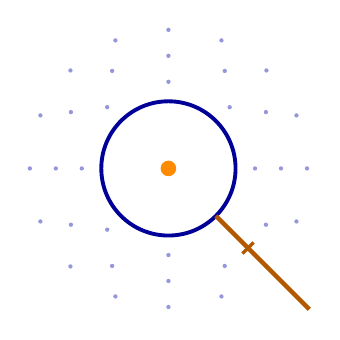
\begin{tikzpicture}[scale=0.55]
% sweep dots forming concentric search rings
\foreach \r/\d in {2.0/8, 2.6/12, 3.2/16}{
  \foreach \i in {1,...,\d}{
    \pgfmathsetmacro{\ang}{(\i/\d)*360}
    \fill[gray!50!blue, opacity=0.55]
      ({\r*cos(\ang)}, {\r*sin(\ang)}) circle (0.05);
  }
}
% magnifier ring
\draw[line width=1.4pt, blue!60!black] (0,0) circle (1.55);
% lens dot
\fill[orange!90!yellow] (0,0) circle (0.18);
% handle
\draw[line width=1.6pt, orange!70!black]
  ({1.55*cos(-45)},{1.55*sin(-45)}) -- ({4.6*cos(-45)},{4.6*sin(-45)});
% binding band
\draw[line width=1.2pt, orange!70!black]
  ({2.6*cos(-45)+0.18*cos(45)},{2.6*sin(-45)+0.18*sin(45)})
  -- ({2.6*cos(-45)-0.18*cos(45)},{2.6*sin(-45)-0.18*sin(45)});
\end{tikzpicture}\\[0.2em]
{\footnotesize\itshape ~AMB \(\cdot\) ORCID 0009-0007-2787-943X
\(\cdot\) v1.0 \(\cdot\) 2026~}
\end{center}

\end{document}
